\documentclass[10pt]{report}
\usepackage{tikz}
\usetikzlibrary{arrows}
\usepackage{natbib}
\usepackage{graphicx}
\usepackage{url}
\usepackage{fancyhdr}
\pagestyle{fancy}


\newtheorem{thm}{Theorem}
\newtheorem{lem}[thm]{Lemma}
\newtheorem{defn}[thm]{Definition}
\newtheorem{ex}[thm]{Example}
%\newtheorem{claim}[thm]{Claim}

%\newcommand{\squash}{\parskip=0ex\itemsep=0ex}
\newcommand{\cnf}[1]{\ensuremath{\operatorname{\mathsf{#1}}}}
\newcommand{\cnc}[1]{\ensuremath{\mathsf{#1}}}
\newcommand{\fnf}[1]{\ensuremath{\operatorname{\mathit{#1}}}}
\newcommand{\fnc}[1]{\ensuremath{\mathit{#1}}}

% Binary operators for linear and branching terms
\newcommand{\linseq}{\prec}
\newcommand{\linpar}{\sim}
\newcommand{\sdup}{\leftrightarrow}
\newcommand{\slft}{\leftarrow}
\newcommand{\srht}{\rightarrow}
\newcommand{\bradupseq}{\stackrel{\sdup}{\linseq}}
\newcommand{\bralftseq}{\stackrel{\slft}{\linseq}}
\newcommand{\brarhtseq}{\stackrel{\srht}{\linseq}}
\newcommand{\braduppar}{\stackrel{\sdup}{\linpar}}
\newcommand{\bralftpar}{\stackrel{\slft}{\linpar}}
\newcommand{\brarhtpar}{\stackrel{\srht}{\linpar}}
\newcommand{\linseqe}{\to}
\newcommand{\braseqe}[1]{\stackrel{#1}{\prec}}
\newcommand{\brapare}[1]{\stackrel{#1}{\sim}}

\newcommand{\ia}{a}
\newcommand{\apdt}{phrase}
\newcommand{\Ia}{A}
\newcommand{\Apdt}{Phrase}

\newcommand{\skp}{\cnc{SKIP}}
\newcommand{\cpy}{\cnc{CPY}}
\newcommand{\done}{\cnc{DONE}}
\newcommand{\at}[2]{\mathop{@_{#1}}{#2}}
%\newcommand{\ati}[3]{\mathop{@_{#1}}[{#2}]{#3}}
\newcommand{\sig}{\cnc{SIG}}
\newcommand{\hsh}{\cnc{HSH}}
\newcommand{\kimc}{\cnc{KIM}}
\newcommand{\kim}[2]{\cnc{KIM}~#1~#2}
\newcommand{\kime}[3]{\cnc{KIM}~#1~#2~#3}
\newcommand{\usm}{\cnc{USM}}
\newcommand{\usme}[1]{\cnc{USM}~#1}

\newcommand{\seqe}{\mathbin{;\!;}}
\newcommand{\pare}{\parallel}
\newcommand{\mt}{\xi}
\newcommand{\sign}[2]{[\![#1]\!]_{#2}}
\newcommand{\hash}[2]{\mathop{\#_{#1}}{#2}}
\newcommand{\KK}[2]{\cnc{K}^{#1}_{#2}}
\newcommand{\UU}[1]{\cnc{U}_{#1}}
\newcommand{\Ke}[4]{\cnc{K}^{#1}_{#3}({#4})}
\newcommand{\Ue}[3]{\cnc{U}_{#2}({#3})}

\newcommand{\eval}[3]{\mathcal{E}({#1},{#2},{#3})}
\newcommand{\aeval}[3]{\bar{\mathcal{E}}({#1},{#2},{#3})}
\newcommand{\evalS}[1]{\ensuremath{\mathcal{E}(#1)}}
\newcommand{\evalv}[3]{\mathcal{V}({#1},{#2},{#3})}
\newcommand{\evalvS}[1]{\mathcal{V}({#1})}
\newcommand{\po}[3]{\mathcal{R}({#1},{#2},{#3})}
\newcommand{\bfr}[3]{{#1}\mathbin:{#2}\prec{#3}}
%\newcommand{\bfr}[3]{{#2}\prec_{#1}{#3}}
\newcommand{\splt}[2]{\mathcal{S}({#1},{#2})}
\newcommand{\subterm}{\sqsubseteq}
\newcommand{\sevalf}{\mathcal{F}}
\newcommand{\seval}[1]{\sevalf({#1})}
\newcommand{\placef}{\mathcal{G}}
\newcommand{\place}[1]{\placef({#1})}
\newcommand{\halt}[1]{\mathcal{H}({#1})}
\newcommand{\size}[1]{|{#1}|}
\newcommand{\evof}{\mathrel\Diamond}
\newcommand\te[4]{{#1}\evof^{#2}_{#3}{#4}}
% for tables
\newcommand\tte[4]{{#1}&{}\evof^{#2}_{#3}{}&{#4}}

\newcommand{\futr}{\cnc{FUTR}}

\newcommand{\nat}{\mathbb{N}}
\newcommand{\anno}[3]{[{#1}]^{#3}_{#2}}
\newcommand{\step}{\leadsto}
\newcommand{\lts}[3]{{#2}\mathbin:{#1}\step{#3}}
\newcommand{\lstp}[3]{{#1}\stackrel{#2}{\leadsto}{#3}}
\newcommand{\nstep}[1]{\leadsto^{{}_{#1}}}
\newcommand{\kstar}{\leadsto^*}
\newcommand{\nlstep}[2]{\stackrel{\!\!#1}{\leadsto^{{}_{#2}}}}
\newcommand{\lstep}[1]{\stackrel{#1}{\leadsto}}
\newcommand{\lstar}[1]{\stackrel{\!\!#1}{\leadsto^{{}_{*}}}}
\newcommand{\nlstar}[2]{\stackrel{\!\!#1}{\leadsto^{{}_{#2}}}}
\newcommand{\sseq}{\mathbin{;}}
\newcommand{\sfut}{\mid}
\newcommand{\qmid}{\mathbin{\mbox{`$\mid$'}}}
\newcommand{\ssft}{\mathbin{;\!;}}
\newcommand{\spar}{\parallel}
\newcommand{\sstop}{\mathcal{D}}
\newcommand{\conf}{\mathcal{C}}
\newcommand{\lseq}{\mathcal{LS}}
\newcommand{\bseq}{\mathcal{BS}}
\newcommand{\bpar}{\mathcal{BP}}
\newcommand{\ats}{\mathcal{A}}

\newcommand{\compf}{\mathcal{C}}
\newcommand{\comp}[2]{\compf({#1},{#2})}
\newcommand{\compp}[2]{[{#2}]_{#1}}
\newcommand{\cop}[1]{\mathbin{\cdot{#1}\cdot}}
\newcommand{\atc}[1]{\mathop{\bar{@}_{#1}}}
\newcommand{\estep}{\Rightarrow}

\newcommand{\seq}[1]{\ensuremath{\langle#1\rangle}}
%\newcommand{\app}{\mathbin{{}^\smallfrown}}
\newcommand{\app}{\mathbin{\ast}}
\newcommand{\cons}{\mathbin{::}}
\newcommand{\sel}{\mathbin{\downarrow}}

\newcommand{\csize}[1]{\ensuremath{\mid\!#1\!\mid}}
\newcommand{\labi}[2]{\ensuremath{\alpha({#1},#2)}}
\newcommand{\lab}[1]{\ensuremath{\alpha(#1)}}
%\newcommand{\tsize}[1]{\ensuremath{\mid\!#1\!\mid}}
\newcommand{\tsize}[1]{\size{#1}}

\newcommand{\term}{\cnc{APDT}}
%\newcommand\tr[4]{{#1}\mathcal{T}^{#2}_{#3}{#4}}
\newcommand\tr[4]{{#1}\mathbin\Box^{#2}_{#3}{#4}}
\newcommand{\trace}[2]{\ensuremath{\mathcal{T}(#1,#2)}}
\newcommand{\traceS}[2]{\ensuremath{\mathcal{T}(#1,#2)}}
\newcommand{\langsc}{\textsc{Copland}}
\newcommand{\lang}{Copland}


\newcommand{\bs}{\cnc{BS}}
\newcommand{\argt}{\cnc{ARG}}
\newcommand{\Uec}[5]{\cnc{U}_{#1}~#2~[#3]~#4~(#5)}
\newcommand{\Kec}[6]{\cnc{K}^{#1}_{#2}~#3~[#4]~#5~(#6)}
\newcommand{\Gec}[3]{\cnc{G}_{#1} \hspace{1mm} #2 \hspace{1mm}  #3}
\newcommand{\Hec}[2]{\cnc{H}_{#1} \hspace{1mm} #2}
\newcommand{\Nec}[3]{\cnc{N}_{#1} \hspace{1mm} #2 \hspace{1mm} (#3)}
\newcommand{\Sec}[2]{\cnc{SS} \hspace{1mm} {#1} \hspace{1mm} {#2}}
\newcommand{\Pec}[2]{\cnc{PP} \hspace{1mm} {#1} \hspace{1mm} {#2}}
\newcommand{\mtc}{\cnc{mt}}

\newcommand{\pl}{\cnc{P}}

\newcommand{\evc}[0]{\cnc{\emph{e}} }
\newcommand{\strj}{\cnc{<string>}}
\newcommand{\numj}{\cnc{<number>}}
\newcommand{\arrj}{\cnc{<array>}}

\lhead{CAPTools Documentation}
\rhead{KU System-Level Design Group}
\lfoot{\copyright The University of Kansas, 2019}
\cfoot{\thepage}

\newtheorem{conjecture}{Conjecture}
\newtheorem{obligation}{Obligation}
\newtheorem{definition}{Definition}

\usepackage[textsize=tiny]{todonotes}
%%\usepackage{ifthen}
% \newboolean{submission}  %%set to true for the submission version

\newcommand{\squash}{\itemsep=0pt\parskip=0pt}
\newcommand{\terms}[0]{\cnc{\emph{t}} }
\newcommand{\req}[0]{\cnc{\emph{R}}}
\newcommand{\nonce}[1]{\cnc{NONCE_{#1}}}
\newcommand{\vals}[0]{\cnc{\emph{e}}}}
\newcommand{\proposal}[0]{$\langle p_0,p_1,\ldots,p_n\rangle$}
\newcommand{\bara}[0]{$\mathit{\bar{a}}$}

\parskip=\medskipamount
\parindent=0pt

\bibliographystyle{abbrvnat}


\title{Certified Attestation Protocol Tools - Version 0.1}
\author{
  Anna Fritz \\
  Information and Telecommunication Technology Center \\
  The University of Kansas \\
  \url{arfritzz@ku.edu}
}

\begin{document}

\maketitle
\tableofcontents

\chapter{Current Focus}

Thinking about situational awareness

Monad to describe the shape of the protocol? 

Layered attestation paper to learn what measures what and system 
capabilities. 
Sufficiency =  What paul and john are talking about in paper
Soundness = Measurement  I took gives me what I want

"Finding scenarios is a job for a model checker" - Adam

\chapter{Design}

\section{Initial Overview}

Negotiation occurs between two parties: the appraiser and the target.
The goal is to gather evidence about a target. The appraiser sends the
target a \textbf{request}. The target then responds
with a \textbf{proposal} which is a set of \textbf{protocols}. The goal of
negotiation is then to select the "best" protocol. However, in order to
choose the "best" from the set, there must be some notion of ordering.
Typically, the best protocol would be the one that relays the most 
information about a system. Therefore, these protocols must all be evaluated
to evidence, then an ordering on evidence must be imposed, then the initial protocols can be ordered. 
In turn, an ordering over protocols will be discovered when all 
protocols are evaluated to evidence.  

\section{Basics}

To begin constructing the language, there are basic things we must implement. 

\begin{itemize}
\item Place = \pl
	\begin{itemize}
	\squash
	\item Formally, any location where attestation protocols are interpreted. 
	\item Each place has a private key and policy
		  identifying how it performs measurements. 
	\item For now, place is a natural number that represents where the
          Negotiation is occurring.  
	\end{itemize}
\item Term = \terms
	\begin{itemize}
	\squash
	\item A term is a Copland term. 
	\item This is useful for the Privacy Policy to decide what terms can
          be shared. 
	\item A Proposal will be composed of a list of terms from the target
          to the appraiser.
	\item I suppose when we go to define an ordering to establish a meet
          and join we will order the terms. This seems like a natural place
          to establish ordering. 
	\end{itemize}
\item Request = \req
	\begin{itemize}
	\squash
	\item A request asks the target for evidence. 
	\item It can ask for one thing, one thing or the other thing, or
          both things. 
	\item Request is an Inductive definition then so that the constructors
          can be `one` `prod` `sum`.
	\end{itemize}
\item Proposal = \proposal
	\begin{itemize}
	\squash
	\item Proposal is a definition (function) which takes a request
          and generates a list of terms
	\item Somewhere somehow the privacy policy must be satisfied. 
	\item Dr. A suggest making a theorem that says "forall protocols,
          the privacy policy is satisfied"
	\item This leads me to ask "How do we write the privacy policy in
          terms of code?"
	\end{itemize}
\item Evidence = \vals
	\squash
	\begin{itemize}
	\item Evidence is produced by protocol execution and results in 
          basic values and compositions operators that indicate order 
	      and place.
	\end{itemize} 
\end{itemize}

Knowing these pieces are needed, an initial step by step procedure can be composed.

\begin{enumerate}
\squash
\item A Request is generated from the appraiser and sent to the target
	\begin{itemize}
	\squash
	\item Request now only composed of one thing.
	\end{itemize}
\item The target looks at the request and responds with the proposal. The
        proposal is a list of protocols. 
\item The appraiser selects a protocol.
\item The protocol is sent to the Attestation Manager.  
\end{enumerate} 

\begin{figure}[hbtp]
  \centering
  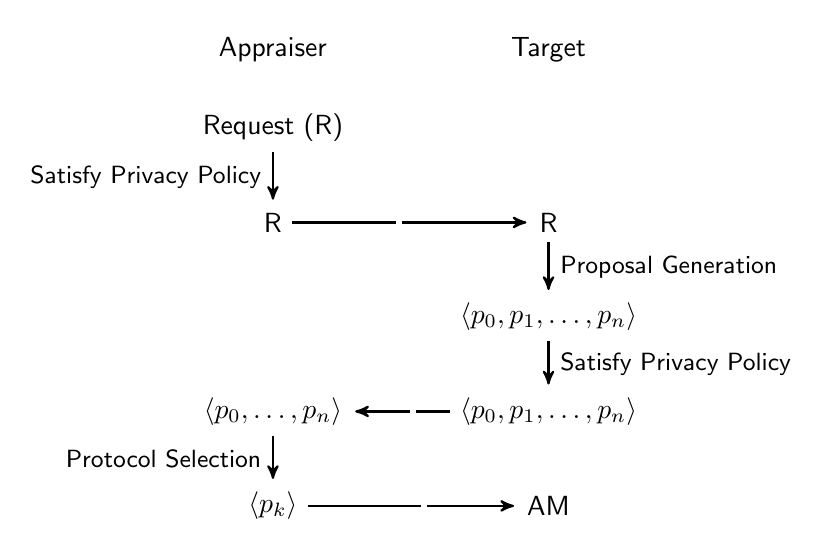
\begin{tikzpicture}[->,>=stealth',shorten >=1pt,auto,node distance=1.2cm,
  thick,main node/.style={rectangle,%%fill=blue!20,draw,
    font=\sffamily,minimum height=2mm,minimum width=2mm}]


  \node[main node] (Request) {Request (R)};
  \node[main node] (AppPrivPol) [below of=Request] {R};
  \node[main node] (R) [node distance=3.5cm, right of=AppPrivPol] {R}; 
  \node[main node] (TarPrivPol) [below of=R] {$\langle p_0,p_1,\ldots,p_n\rangle$}; 
  \node[main node] (TarProp) [below of=TarPrivPol] {$\langle p_0,p_1,\ldots,p_n\rangle$};  
  \node[main node] (AppProp) [node distance=3.5cm, left of=TarProp] {$\langle p_0,\ldots,p_n\rangle$};
  \node[main node] (Protocol) [below of=AppProp] {$\langle p_k\rangle$};
  \node[main node] (AM) [node distance=3.5cm, right of=Protocol] {AM}; 
  \node[main node] (IN) [node distance=1.0cm, above of=Request] {Appraiser};
  \node[main node] (OUT) [node distance=3.5cm, right of=IN] {Target};
    

  \path[every node/.style={font=\sffamily\small, fill=white,inner sep=1pt}]
    (Request) edge node[left=1mm] {Satisfy Privacy Policy} (AppPrivPol)
    (AppPrivPol) edge node[left=1mm] {} (R)
    (R) edge node[right=1mm] {Proposal Generation} (TarPrivPol)
    (TarPrivPol) edge node[right=1mm] {Satisfy Privacy Policy} (TarProp)
    (TarProp) edge node[right=1mm] {} (AppProp)
    (AppProp) edge node[left=1mm] {Protocol Selection} (Protocol)
    (Protocol) edge node[right=1mm] {} (AM)	
	;
\end{tikzpicture}

%%% Local Variables: 
%%% mode: latex
%%% TeX-master: "certification"
%%% End:

  \caption[Attestation and Appraisal Sequence for One Request]{Processing sequence for
    Negotiation, Selection, Attestation and Appraisal during remote
    attestation.}
  \label{fig:att-app-seq}
\end{figure}

\section{Situational Awareness}

Situational Awareness can be described as the program's understanding of
the urgency of measurement and the level of detail of measurement that
must be achieved. For example, if the situation is an aircraft flying
over a radio tower, the airplane is quick so attestation must be preformed
quickly. This situation would not allow much time for negotiation. However,
if someone from the NSA needed information about the whole network and to
make sure each component had up-to-date software, this person would want
the attestation preformed in a reasonable amount of time but would not
need it quickly. They might be more interested in having fresh and
detailed evidence.

With those examples, it is evidence there must be some component of
Negotiation that is situationally aware. That is, understands the
timing, freshness, and level of detail that the attester demands.
It is then imporatant to understand the key details that will allow
for concise situational awareness.

\begin{enumerate}
\item Time stamp = something that communicates the urgency or
  ease of the situation.
\item Freshness = a key parameter that details if the appraiser
  is willing to accepted old, cached results or if the appraiser
  demands new protocols.
\item Desired level of detail = this fact I am the most unsure
  about as at some point, the appraiser must decide a ranking
  of the protocols and the length of each list of terms in each
  protocol seems like an intrinsic place to start. We can order
  the protocols by the evidence produced but then again, does the
  appriser want the longest or shortest protocol? Maybe in some
  situations they will opt for the shortest protocol. 
\end{enumerate}


The most logical place for this to fit appears to be in the request.
If one wants to communicate quickly, it is not necessary for the target
to generate a hash of every file it has but rather a hash of only one
file, for times sake. 

\section{Privacy Policy}

At this point, the privacy policy is a filter for the target and appraiser, where 
information passes through the filter before it is exchanged between parties. 
Both the appraiser and the target have their own, unique
privacy policies. Also, in more general terms, each computer or cluster
must have a privacy policy as a target and as an appraiser so that it
can morph between the two roles. 

Who communication will occur between, be it a network of computers or
one single computer, will be established in the Security Association.
Once that is established, the privacy policy may change to reflect
the communication based on the role of target or appraiser. 

\section{Ideal trust establishment function}

The ideal trust establishment $\delta_m:R\rightarrow (E,\preceq,\top,\bot)$ ,
or $\delta_m$. 

$\delta_m$ relates a request to the set of all evidence packages that 
could result from that request.  Those evidence packages are ordered
by $\preceq$ that defines relative``quality'' of evidence.  If
$e_1\preceq e_2$ then evidence $e_2$ is of higher quality than $e_1$.
Quality is subjective and this order reflects situational awareness.
The relation $\preceq$ is by definition a partial order 
over evidence while $\bot$ and $\top$ are the worst and best evidence
corresponding to no description and an exact description
respectively.  This defines a bounded lattice, however more work is
needed to establish the correctness of the approach.

$\gamma_n$ produces a proposal $\langle p_0,p_1,\ldots,p_n\rangle$
from a request, $r$ based on target policy. $\delta_c$
transforms the proposal into evidence from each protocol,
$\langle e_1,e_2,\ldots,e_n \rangle$. Thus $\delta_c$ is a functor
over proposals---vectors of protocols---to vectors of evidence.
$\alpha_n$ lifts the evidence vector into the evidence lattice.

\section{Request}

\subsection{ISAKMP}
  
One feature of the Request that it must be situationally
dependent. For example, if the apprasier is a UAV flying over a
groundstation, then they want to preform attestation quickly and thus
need a quick negotiation procedure. One way to do this is through the
implementation of ISAKMP. With ISAKMP, not only are naming semantics
and crytography features agreed upon, but also a notion of promptness can
be asserted by the SA. 

\subsection{Request Composition}
  
  Right now the exact understanding of the Request is not important.
  Only a general understanding in needed and useful. 
  
  A request is composed of some sort of evidence. It can be three things:
  \begin{enumerate}
  \squash
  \item one evidence
  \item sum of evidence (OR)
  \item product of evidence (AND)
  \end{enumerate}

  
  Some other parameters that must be taken into consideration when
  requesting information is: 
  
  \begin{itemize}
   \squash
   \item place
   \item the appraiser privacy policy
   \item ISAKMP
   \end{itemize}

\section{Proposal}

\subsection{Producing a proposal}

A proposal is a set of protocols generated by the target upon receiving
the target's request. Therefore, the proposal takes in the appraiser's
request and returns a list of terms. The coq definition for this may
look something like an interpeter: 
  
\begin{verbatim}
  
  Definition propose : (request ev) -> list term

\end{verbatim}  
  
  In this definition, the appraiser receives a list of terms. The list
  of terms must satisfy the privacy policy for the target before being
  sent to the appraiser. In the future, some things that should be
  considered in the proposal are:
  
  \begin{itemize}
   \squash
   \item the target's privacy policy
   \item ISAKMP
  \end{itemize}
  
  The proposal can be ordered or unordered, it does not really
  matter. The appraiser decides the ordering so the appraiser orders
  the set before selection.

\subsection{Shape of a Protocol}

A protocol is a phrase (T) parameterized by atomic axioms (A).
The protocol can suggest the action be preformed at the assoicated place
(measure the local environment), or measure another place. These
measurements can be taken in sequence or parallel. There are two types of sequence
calculations, the first is where the first term is input
to the second term dicatated by $(t \linseqe t)$.
When doing this evaluation, the first term runs to compeltion
before the second term begins. The other kind of linear evaluation
differs in that evidence is not send from the
first term as input to the second term, rather each term recieves some
filtered version of evidence accumulated from the parent phrase. This
is represented with $(t\braseqe\pi t)$. Finally, two
subterms can be execued in parallel with data splitting,
represented by $(t\brapare\pi t)$. In the final two cases, $\pi$ is the
data splitting function that dictates how evidence is split
between two subterms. 

\section{Selecting a Protocol}

  The function, ($\gamma_{n}$), selects a protocol $(P_{k})$ 
  from a proposal $\langle p_0,p_1,\ldots,p_{n}\rangle$.  

  The selection of a Proposal will involve ensuring that the chosen
  protocol meets the initial negotiation condition. This can be
  represented in an Inductive definition as follows:
  
  \begin{verbatim}
  Inductive negotiationR : Request -> Place -> term -> Prop :=
  | n1 : (ev1) -> n -> (USM 1) -> True
  .
  .
  .
  . where one can list various options for negotiation. 
  \end{verbatim} 
  
  The selection of a proposal has been greatly discussed. The
  appraiser will always select the best proposal, but how? There must be some
  type of ordering on the members of the set that established a notion of
  "best." This is how a lattice comes into play. Within a lattice, the is
  some sort of ordering. Therefore, each unique system will produce its own
  notion of ordering allowing for there to then be a best and worst protocol
  in each set. 
	
  The lattice definition is tricky because we cannot list out cases as
  seen in the example because each system is different. Instead, we must
  keep it more general. 

\subsection{Creating a Map for Requests to Protocols}
  
In order to evaluate a request, there must be some sort of value that
the request constructors evaluate to. This way of storing values lends
itself to a Map where elements are placed into the data structure in
key/value pairs. To get the value, the user supplies the key and the
dictionary returns the value.

If the lookup key is not in the table, the map should return an empty
default element. 
  
\section{Evaluating Proposal}

Evaluating a proposal will occur in the Attestation Monad. The job of
Negotiation is simply to choose a protocol that will be evaluated. It is
important to note, however, the result of evaluating a proposal is evidence
about the system. 

\chapter{Copland Language Specifications}

\section{Copland Language Basics}

In defining Copland, two forms of semantics were written: 
denotational, and event-based operational. First, denotational 
semantics maps the terms to the evidence they produce. 
The event-based operational semantics defines the system 
of events associated with the protocol execution. 

In order to understand the semantics, one must understand 
the syntax surrounding Copland. Below is a list of Copland 
syntax to aid in comprehension. 

\begin{itemize}
\squash
\item Terms (or phrases) $=$ individual protocols 
\item Evidence $=$ the form of evidence produced by protocol 
      execution
\item P $=$ Place or location where attestation protocols 
	are interpreted. Each place has a unique private key
	and policy to identify how it preforms measurement
\item (USM  a)
    \squash
	\begin{itemize}
	\item USM $=$ User Space Measurement that preforms 
	measurement in the local user space
	\item measurement details $=$ $\mathit{\bar{a}}$ $=$ Abstractly represents 
	the details of the measurement operation
	\end{itemize}
\item (KIM $\mathit{P \bar{a}}$)
	\squash
	\begin{itemize}
	\item KIM $=$ Kernel Integrity Measurement that 
	examines some external system
	\item measurement details $=$ \textit{a} $=$ abstractly represents 
	the measurements operation
	\end{itemize}
\end{itemize}

\section{Measurement Operations}

There is no merit in defining Copland if one does not 
explain the language's measurement capabilities. 
Those capabilities are as follows:

\begin{itemize}
\squash
\item Hashing a file
\item Requesting a TPM quote
\item Examining the local/proc directory contents
\end{itemize} 

The minimal set of evidence operations includes 
CPY, SIG, HSH which parse to copying, singing 
and hashing evidence values, respectively. 

\section{Evidence Values}

The result of protocol execution produces evidence 
values. These values are represented by $\varepsilon$, 
or the empty set, $U_p(E)$, or the evidence value 
produced by a USM, and $K_Q^P(E)$, or the evidence 
result of a KIM of place P preformed by place Q. 

\section{Evidence Semantics}

Figure~\ref{fig:evidence-semantics} defines a denotational semantics,
$\eval{t}{p}{e}$, mapping each Copland term, $t$, initial evidence
value, $e$, in some place, $p$, to a resulting evidence term. In the formal
Copland specification this is called the \emph{evidence semantics}, and
it provides a requirements definition for Copland interpreters. 

\newpage

\begin{figure}
  \begin{eqnarray*}
    \eval{\usme{\bar{a}}}{p}{e}&=&\Ue{\bar{a}}{p}{e}\\
    \eval{\kim{q}{\bar{a}}}{p}{e}&=&\Ke{q}{\bar{a}}{p}{e}\\
    \eval{\cpy}{p}{e}&=&e\\
    \eval{\sig}{p}{e}&=&\sign{e}{p}\\
    \eval{\hsh}{p}{e}&=&\hash{p}{e}\\
    \eval{\at{q}{t}}{p}{e}&=&\eval{t}{q}{e}\\
    \eval{t_1\linseqe t_2}{p}{e}&=&\eval{t_2}{p}{\eval{t_1}{p}{e}}\\
    \eval{t_1\stackrel{\pi}{\linseq} t_2}{p}{e}&=&\eval{t_1}{p}{\pi_1(e)}\seqe
      \eval{t_2}{p}{\pi_2(e)} \\
    \eval{t_1\stackrel{\pi}{\linpar} t_2}{p}{e}&=&\eval{t_1}{p}{\pi_1(e)}\pare
       \eval{t_2}{p}{\pi_2(e)} \\
    & & \mbox{ where $\pi=(\pi_1,\pi_2)$}
  \end{eqnarray*}
  \vspace{-1ex}
  \caption{Evidence Semantics.}
  \label{fig:evidence-semantics}
\end{figure}

\section{Ordering Evidence}

Evidence is ordered by the notion of "best." "Best" in this case is 
situationally dependent and therefore depends on many varying 
characteristics of the system. 

\begin{itemize}
  \squash
  \item Most difficult for an attacker
  \item Most detailed response for the appriaser
  \item Longest or shortest time depending on situational awareness
\end{itemize}

Therefore, there are too many variable to uniquely cover
each situation that could arise. Therefore, we must understand
the types of information necessary to make the "best" decision. 
Perhaps the best way to know what characteristics may lend
themselves to the notion of "best" is with the "Principles of Remote 
Attestation" paper by Coker et al. In that paper, the authors define
five principles of attestation architectures. They are as follows: 

\begin{enumerate}
  \item Fresh Information
	\begin{itemize}
	\item Is the appraiser willing to accepted a cached result?
	\item How will we keep a time stamp on the evidence collected?
	\end{itemize}
  \item Comprehensive Information
	\begin{itemize}
	\item Is the best evidence the one with the most information? 
		  The target wants to avoid giving away too much information
		  while the appraiser wants as much as possible. Does the
          notion of "best" fit somewhere in the middle?
	\item The space concern: does having too much information mean 
          consuming too much space in memory?
	\item How long is the appraiser willing to wait? If the request
		  is large enough that it takes the target a while to generate
          the proposal, what would be the maximum time limit?
	\end{itemize}
  \item Constrained Disclosure
	\begin{itemize}
	\item Appraiser must be identifiable to the target. How should 
		  we include some kind of label? A hash? 
	\item Both Target and Appraiser policies must be included working
		  to satisfy the appraiser's desire for disclosure and the
		  target's desire for privacy. 
	\end{itemize}
  \item Semantic Explicitness
	\begin{itemize}
	\item States semantics are presented in logical form so that appraiser
          can infer consequences of attestations. 
	\end{itemize}
  \item Trustworth mechanism
	\begin{itemize}
	\item The attestation architecture should be identified to the target
		  and the appraiser. 
	\end{itemize}
\end{enumerate}

From these five principles, one can develop a notion of "best."

There are also five main constraints that are motivated by the priniples,
as listed below. A system, therefore, must have the following abilities:

\begin{enumerate}
	\item Measure
	\item Separate domains
	\item Protect itself
	\item Delegate attestation
	\item Manage attestation
\end{enumerate}

\chapter{ISAKMP/IKE} 

In general, Internet Security Association and Key Management Protocol
(ISAKMP) is the protocol that establishes Security Associations
(SA) and cryptographic keys outlined in RFC 2408. There are
four main goals of ISAKMP which include authenticating a communicating
peer, creation and management of security associations, key generation techniques,
and threat mitigation. In summary, the goal of ISAKMP is for transferring keys
and authenticating data. 

In terms of authenticating a communicating peer, ISAKMP encourages
strong authentication through the use of a security association (SA). The SA is defined 
as a relationship that describes how the entities will utilize security services to 
communicate securely. The procedure
outlined in ISAKMP allows an entity's initial
communications to indicate which certificate authorities (CAs) it supports.
In creating and managing the security association, one side must assume the role
of initiator and the other assumes the role of responder. Proposal and
transform payloads are then exchanged to establish the security association.
Also, ISAKMP provides key generation techniques that enforce  authentication
of key exchange, key exchange symmetry and perfect forward secrecy. The specifics
of key generation and transport is outlined in IKE. Finally, ISAKMP enforces
threat mitigation techniques by addressing the prevention of possible attacks
such as anti-clogging, connection hijacking, and man-in-the-middle attacks.
It is important to note that ISAKMP sets up security associations and then 
provably does not alter the security associations during run-time. Instead,
the SA's become read-only. 

There are a few other concepts from ISAKMP that are important to note.
First, and entity's name is its identity where the agreed upon certificate
authority defines the naming semantics. Once the certificate the verified,
the name is verified, and then the name has meaning within the
certificate authority. Also, the domain of interpretation (DOI) defines the
situation and set of security policies that may be supported. It also houses
additional exchange types, a scheme for naming security-relevant information,
key exchange algorithms, security policy attributes, and certificate authorities. 

Furthermore, once a SA is created, it would be help to be able to reference the 
SA at a later date. With that, a Security Parameter Index (SPI) is an identifier 
specifically for Security Associations. A SPI pair may uniquely identify a SA but 
the SPI implementation is dependent on the DOI. The DOI determines which SPIs
are sent during communication.

\section{What ISAKMP Communicates}

In general, ISAKMP establishes security associations (SA) between two communicating
parties. Below are the characteristics of a SA that are agreed upon by the Target and 
the appraiser. 

\begin{itemize}
  \item Which certificate authority the entity supports
  \item Naming semanitcs
  	\begin{itemize}
	\item The name has meaning within the certificate authority
          when the name is verified. 
	\end{itemize}
  \item Domain of Interpretation (DOI)
  	\begin{itemize}
	  \item Defines payload formats
	  \item Defines exchange type
	  \item Defines a scheme for naming security-relevant
            information ie naming information
	\end{itemize}
\end{itemize}

\section{How it works}

\begin{enumerate}
  \squash
              \item ISAKMP Header = provides information required by the protocol to
                maintain association throughout communication.
              \item Generic Payload Header = chains several payloads together and allows
                for the protocol 
    		to remain flexible
              \item Security Association Payload = convey the security attributes to be
                used in establishing
  		the SA
		\begin{itemize}
		\squash
		\item DOI identification is included here
		\end{itemize}
              \item Proposal Payload = various information associated with the security
                relationship
  		\begin{itemize}
		\squash
	      \item Populated with transform payloads that contain the SA
                information
	      \item Initiator sends proposal payload with one or more trans
                form payloads within each that define available security conditions
	      \item Responder selects the proposal and associated transform
                         sets that best pertain
			 to the communication
		\end{itemize}
\end{enumerate}

\section{ISAKMP/IKE Results}

ISAKMP creates a SA between two communicating peers. In order to do this,
the peers must agree on policies. Once the initator and responder agree
on policies, a SA is established with a time stamp. Those agreed policies
can then be used for further communication. Those policies are seen below (2):

\begin{itemize}
  \squash
\item an authentication method (ensure id of peers)
  \begin{itemize}
 \squash
\item rsa-sig = digital certificate with keys generated by RSA signature
  algorithm
  \item crack = challenge/response for authenticated cryptographic keys
  \item pre-share (default) = preshared keys
  \end{itemize}
\item an encryption method (protect data and ensure privacy)
  \begin{itemize}
 \squash
  \item des = 56-bit DES-CBS
  \item 3des (default) = 168-bit Triple DES
  \item aes = advanced encryption standard supports lengths 128, 192, 256 bits
  \item aes-192
  \item aes-256  
  \end{itemize}
\item Hashed Message Authentication Codes (HMAC) (ensure message has not
  been modified in transit)
  \begin{itemize}
 \squash
  \item sha (default) = SHA-1 (HMAC variant)
  \item md5 = MD5 (HMAC variant)
  \end{itemize}
\item a Diffie-Hellman group to determine strength of the encryption-key-
  determination algorithm
  \begin{itemize}
 \squash
  \item 1 = Group 1 (768-bit)
  \item 2 = Group 2 (1024-bit)
  \item 5 = Group 5 (1536-bit)
  \item 7 = Group 7 (Elliptical curve field size is 163 bits)
  \end{itemize}
\item a limit to the time the SA is valid
  \begin{itemize}
 \squash
  \item integer value (86400 is default) = 120 to 2147483647 seconds
  \end{itemize}
\end{itemize}

Also, the ISAKMP header contains a SA payload that contains the domain of
interpetation (DOI) and the situatuion. 

\section{ISAKMP Dictionaries}

In order to store the components from the ISAKMP security association (SA)
a dictionary will need to be created that houses the input values from the
communication and translates them into phrases in the Negotiation language.
The first thing to do then is to understand the result of ISAKMP/IKE
contains a SPI, an IP destination address and the security protocol. The
SPI identifies the SA. I imagine this is useful for labeling and
referencing past communications.  

\section{Works Cited}

\begin{enumerate}
\item  
	\begin{verbatim} 
	https://books.google.com/books?id=w2u6a_NZr_8C&pg=PA164&lpg=PA164&dq=ISAKMP+header&source=bl&ots=x45AtA8F2x&sig=ACfU3U3zxANfosIM-H-jKpBOKrrXsHxyxg&hl=en&sa=X&ved=2ahUKEwir_IeR3IDkAhXZW80KHczVD0YQ6AEwE3oECA8QAQ#v=onepage&q=ISAKMP%20header&f=false
	\end{verbatim}
\item
        \begin{verbatim}
        https://www.cisco.com/c/en/us/td/docs/security/asa/asa72/configuration/guide/conf_gd/ike.pdf 
        \end{verbatim}
\end{enumerate}

\chapter{Verification}

\section{Introduction to the Formal Verification of Negotiation}

Before constructing the negotiation procedure, formal verification must occur
to ensure the process achieves the desired results. That is, that the Target
and the Appraiser's privacy policy is met and that the negotiation policy
produces an acceptable protocol for attestation. For negotiation, the architecture
design follows a specific procedure that differs from the systems verification
procedure. This is because the implementation of negotiation will differ from the
verification of negotiation. The procedure for the system's implementation can
be seen in the following list below. 

\begin{enumerate}
\item A request is sent by the Appraiser to the Target. The request must not
  violate the Appraiser's privacy policy. More detailed information about the
  Request can be found in the earlier section. 
\item The Target receives the request and generates a set of protocols also
  known as a proposal. Each protocol must satisfy the Target's privacy policy
  for each Request. 
\item The proposal is sent from the Target to the Appraiser.  
\item The Appraiser orders the set of protocols and chooses the "best" protocol.
  Multi-step negotiation may also occur but that will be discussed later. 
\item The Appraiser sends the "best" protocol through attestation where the
  protocol generates evidence about the system. 
\end{enumerate}

Before the architecture is enforced, there must be formal verification of the
negotiation system. This ensures the procedure is sound and complete. More
importantly, through verification, a notion of "best" protocol is able to be
developed and understood. The verification diagram, as seen below, details
the entire system certification from negotiation through attestation. However,
the concern here is with verification of the negotiation procedure. The
following steps, as outlined below, detail how verification of negotiation
will be accomplished.  

\begin{enumerate}
\item A request is sent by Appraiser to the Target.
\item The Target generates a proposal which is a set of protocols.
\item All generated protocols in the set are evaluated, through attestation,
  to evidence. 
\item The resulting set of evidence is then ordered where "best" is the evidence
  that is the most descriptive of the system and "worst" is the least descriptive
  evidence. 
\item The resulting lattice of evidence is then mapped back to the original set
  of protocols. 
\item The original set of protocols, known as the proposal, now has an ordering
  with the "best" protocol generating the most descriptive piece of evidence.
\end{enumerate}

This verification procedure can then be completed multiple times to gain
a complete understanding of the system and possible negotiation situations.
In the end, a look-up table will be developed that is composed of the possible
protocols and their ordering. 

\begin{figure}[hbtp]
  \centering
  \begin{tikzpicture}[->,>=stealth',shorten >=1pt,auto,node distance=2.0cm,
  thick,main node/.style={rectangle,%%fill=blue!20,draw,
    font=\sffamily,minimum height=7mm,minimum width=10mm}]

\node[main node] (Request) {$R$};
\node[main node] (Result) [node distance=3.0cm, right of=Request] {$(E,\preceq,\top,\bot)$};
\node[main node] (Proposal) [below of=Request] {$\langle P\rangle $};
\node[main node] (ProposalVec) [node distance=3.0cm, right of=Proposal] {$(P,\preceq,\top,\bot)$};

\path[every node/.style={font=\sffamily\small, fill=white,inner sep=1pt}]
  (IN) edge (Request)
  (Request) edge node[below=1mm] {$\delta_m$} (Result)
  (Request) edge node[left=1mm] {Negotiation ($\gamma_{n}$)} (Proposal)
  (Result) edge [dashed] node[below=1mm] {} (ProposalVec)
  (ProposalVec) edge [dashed] node[left=1mm] {} (Proposal)
  (Result) edge (OUT)

\end{tikzpicture}

  \caption[Relational Figure]{ Relational diagram revealing the request,
    evidence, and protocols. The relation between  Solid lines
    represent implementations while dashed lines represent
    mathematical relations.}
  \label{fig:certification-fig}
\end{figure}

The negotiation verification does align with the overall certification task.
However, the two do follow a different structure as the overall certification
involves the hardware implementations. 

\begin{figure}[hbtp]
  \centering
  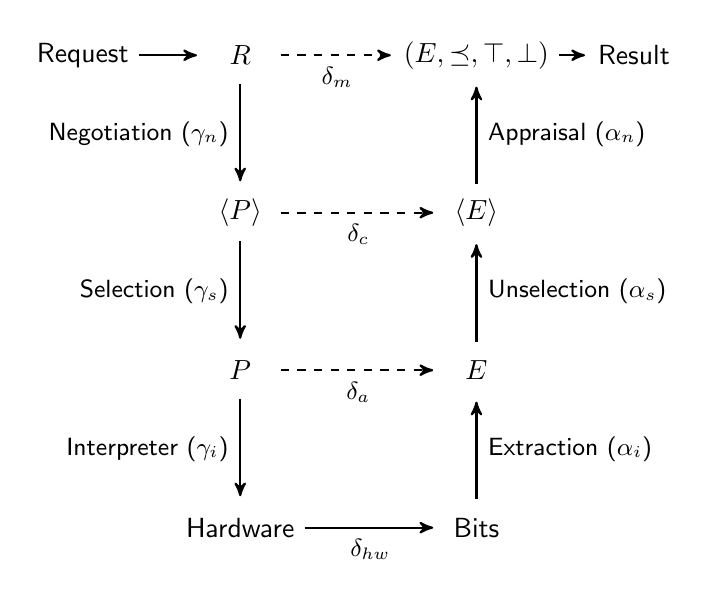
\begin{tikzpicture}[->,>=stealth',shorten >=1pt,auto,node distance=2.0cm,
  thick,main node/.style={rectangle,%%fill=blue!20,draw,
    font=\sffamily,minimum height=7mm,minimum width=10mm}]

  \node[main node] (NM) {$R$};
  \node[main node] (AM) [below of=NM] {$\langle P\rangle $};
  \node[main node] (CP) [below of=AM] {$P$};
  \node[main node] (HW) [below of=CP] {Hardware};
  \node[main node] (HWE) [node distance=3.0cm, right of=HW] {Bits};
  \node[main node] (CPE) [node distance=3.0cm, right of=CP] {$E$};
  \node[main node] (AME) [node distance=3.0cm, right of=AM] {$\langle E\rangle$};
  \node[main node] (NME) [node distance=3.0cm, right of=NM]
  {$(E,\preceq,\top,\bot)$};
  \node[main node] (IN) [node distance=2.0cm, left of=NM] {Request};
  \node[main node] (OUT) [node distance=2.0cm, right of=NME] {Result};
    

  \path[every node/.style={font=\sffamily\small, fill=white,inner sep=1pt}]
    (NM) edge [bend left=0] node[left=1mm] {Negotiation ($\gamma_{n}$)} (AM)
    (AM) edge [bend left=0] node[left=1mm] {Selection ($\gamma_{s}$)} (CP)
    (CP) edge [bend left=0] node[left=1mm] {Interpreter ($\gamma_{i}$)} (HW)
    (HW) edge node[below=1mm] {$\delta_{hw}$} (HWE)
    (CP) edge [dashed] node[below=1mm] {$\delta_a$} (CPE)
    (AM) edge [dashed] node[below=1mm] {$\delta_c$} (AME)
    (NM) edge [dashed] node[below=1mm] {$\delta_m$} (NME)
    (IN) edge (NM)
    (NME) edge (OUT)
    (HWE) edge node[right=1mm] {Extraction ($\alpha_i$)} (CPE)
    (CPE) edge node[right=1mm] {Unselection ($\alpha_s$)} (AME)
    (AME) edge node[right=1mm] {Appraisal ($\alpha_n$)} (NME)
    ;
\end{tikzpicture}

%%% Local Variables: 
%%% mode: latex
%%% TeX-master: "certification"
%%% End:

  \caption[Certification Figure]{Certification stack showing
    certification dependencies and execution path. Solid lines
    represent implementations while dashed lines represent
    mathematical definitions.}
  \label{fig:certification-fig}
\end{figure}

\section{Request}

The request, as previously mentioned, can contain one item, a sum of
items or a product of items. With that, I think we must prove things
about properties of the request.

\begin{itemize}
\item Commutative $ a + b = b + a $
\item Associative $ (a + b) + c = a + (b + c) $
  \begin{itemize}
  \item Order of evaluation matters so I think we need this one.
  \end{itemize}
\item Distributive (I am thinking useful for places maybe?)
  $ (a x (b + c)) = (a x b) + (a x c) $
\end{itemize}

\section{Relationship between Request and Proposal}

A request is comprised of ONE term a SUM of terms or a PROD of terms.
Therefore, the request most likely aligns with a set. One term is just
that, it is its own term. A SUM of terms is a set of individual terms with the
or operator applied to it. A PROD of terms is a set of individual terms
with the and operator applied.

Lets consider the base case; an individual evidence term. We must first
apply our knowledge of the Request leading to a Proposal to a mathematical
data structure to know what is necessary to prove. A morphism is a structure-
preserving map from one mathematical structure to another one of the same type.


\section{Evidence}

Overall, the goal of Copland, and the result of negotiation is preforming
layered attestations which provides
an appraiser with evidence about the integrity of a target. In order to obtain
a protocol from negotiation, however, a notition of "best" protocol must
be implemented. The "best" protocol will be discovered by ordering the
possible evidence values that can arise from processing the protocols. 

\subsection{The Shape of Evidence}

As protocols are evaluated to evidence, there is a natural shape that
arises.

\chapter{Examples}

Throughout the process of understanding negotiation, there are many
examples that have helped me get a better grasp on Coq and what Negotiation
entails. 

\section{The Fruit Example: understanding constructing values}

Let Fruit be a set such that Fruit = { apple , orange , pear }. Then an
inductive data structure for Fruit could read:  

\begin{verbatim}
Inductive request : Type := 
 | one n -> fruit
 | prod fruit -> fruit -> fruit
 | sum fruit -> fruit -> fruit.
\end{verbatim}

Where prod is equivalent to the boolean condition AND and sum is equivalent
to the boolean condition OR. Then creating examples of this would look like: 


(one apple)

(prod (one apple) (one pear))

(sum (one apple) (one pear))

(prod ((prod (one apple) (one pear)) one apple)


Therefore, one apple is a constructing value. It creates a new element that is
now part of the data structure. Overall, this Inductive definition of Request
is a "little language."

Then, generalizing this to all data type we consider the problem of wanting
to use the request data struct for a McDonald's order. If the structure was
untyped, then one could just request an order. To do this, implement the
following structure. 

\begin{verbatim}
Inductive request (ev : Type) : Type :=
| one n -> ev
| prod ev -> ev -> ev
| sum ev -> ev -> ev
\end{verbatim}

\section{Working Example}

The first thing that occurs is a Security Association is agreed up.
Lets say these parameters result from the creation of a security
assoication:

\begin{itemize}
\item rsa-sig = policy authentication
\item des = policy encryption
\item sha = policy hash
\item 2 = policy group (1024-bit DH algorithm)
\item 120 = policy lifetime (seconds)
\end{itemize}

Somewhere, the appraiser must decide on the notion of best. Best is
situationally dependent so lets say for this case best is protocol
with that could be produced the quickest. 

The next thing that occurs is the appraiser must send a request.
For simplicity, lets say the request is a hash of the virus checker. In
copland, this term would look like:

\req $=$ @_{p}\mathsf{USM} \bara

where $\bara$  is a  $\hsh{virus checker}$
so $\req$ $=$ $@_{p}\mathsf{USM}$ $\hsh{virus checker}$

The resulting proposal could then include three options where the first
is a hash of the virus checker, the second is a hash of the virus checker
and a hash of the signature file, and the third option is a hash of the
virus chekcer, a hash of the signature file, and a hash of another piece
of evidence (some component of the network communication). 

The resulting proposal \proposal could then include the following options:

\begin{enumerate}
  \squash
\item Target hashes the virus checker, signs the hash, then sends the
  whole thing back
\item Target can hash the signature file and hash the virus checker
  then send that back
\item Target can hash the virus checker, the signature file, and another
  piece of evidence where the other evidence somehow relies on the network
  connection
\end{enumerate}

or: 

\begin{itemize}
  \squash
\item p_0 $=$ $\mathsf{USM} \hsh{virus checker}$
\item p_1 $=$ $\mathsf{USM} {\hsh{virus checker}, \hsh {signature file}}$
\item p_2 $=$ $\mathsf{USM}$ {$\hsh{virus checker}$, $\hsh {signature file}$},
  additional evidence
\end{itemize}


The proposal is then sent through the privacy policy to ensure that
all options are in alignment with the target's standards.

Then selection procedure is based on situational awareness. Becuase the
situation mandates a response in the shortest amout of time, p_0 will be
favorable. Therefore,\mathsf{USM} \hsh{virus checker} is choosen as the
given protocol to be sent to the attestation manager.

The appraiser then applies the notion of 'best' to the proposal to obtain
the first protocol as the one sent through attestation.

\chapter{Questions:}

About Coq Verification:

\begin{enumerate}
  \item What does the certificate authority get us? A secure channel but 
        does it say anything about the appraiser or target's
        privacy policy?
  \item How does the request generate a proposal? 
  \begin{itemize}
    \item Could think of a request as a condition like all even numbers.
    \item Then Proposal consists of many different sets composed of even
          and odd numbers with each set having varying amounts of numbers.
    \item Then what filters the set to include only even numbers?
          Is that $\delta_c$?
    \item $\delta_c$ is a functor that transforms proposals into evidence.
          I don't really understand this at all.  
  \end{itemize}
  \item Is the targets response, the proposal, an ordered list?
        I think we need a function to ensure ordering.
  \item How are we going to label events? With signing?
  \item What that Appraiser is willing to accept?
	\begin{itemize}
	\squash
	\item The target might not respond with exactly what the appraiser
          had asked for. What is the procedure in that case?
	\item Do we accept other things? Or only what is specifically asked for?
	\item Somewhere their might be a flag that states if ONLY exact is
          acceptable but otherwise, the appraiser must list what is acceptable. 
	\end{itemize}
\end{enumerate}

About Evidence Generation:

\begin{enumerate}
  \item The shape of evidence is discussed in Adam's paper. 
		Is there no notion of actual evidence? Only the shape?
\end{enumerate}

About ISAKMP

\begin{enumerate}
\item What do we need to include in the dictionary?
\item How does the dictionary work?
\item What comes out of ISAKMP?

\end{enumerate}

\end{document}

